% ============================================================================
%  Organisms Write Their Own Evolution
%  arXiv preprint version -- single-author submission
%
%  Build:  make        (or: latexmk -pdf main.tex)
%  Clean:  make clean
% ============================================================================

\documentclass[11pt]{article}

\usepackage[margin=1in]{geometry}
\usepackage[utf8]{inputenc}
\usepackage[T1]{fontenc}
\usepackage{lmodern}
\usepackage{microtype}
\usepackage{amsmath,amssymb}
\usepackage{graphicx}
\usepackage{booktabs}
\usepackage{caption}
\usepackage{authblk}
\usepackage[authoryear,round]{natbib}
\usepackage{xcolor}
\usepackage[colorlinks=true,allcolors=blue,breaklinks=true]{hyperref}

\graphicspath{{figures/}}
\bibliographystyle{plainnat}

\captionsetup{font=small,labelfont=bf}
\setlength{\parskip}{0.35em}
\linespread{1.08}

% --- Convenience macros -----------------------------------------------------
\newcommand{\Pheno}{\textsc{Phenopoiesis}}
\newcommand{\note}[1]{\textcolor{red}{[#1]}}

% ============================================================================
\title{\bfseries Organisms Write Their Own Evolution:\\
Direct Epigenomic Inheritance Accelerates Learning\\ on Compositional Tasks}

\author{Nam H. Le\thanks{Corresponding author: \texttt{namlehai90@gmail.com}}}
\affil{Vermont Complexity Center, University of Vermont, Burlington, VT, USA}

\date{\today}

\begin{document}
\maketitle

% ============================================================================
\begin{abstract}
\noindent
What if organisms could write their own evolution? For 150 years, evolution has been
understood as one-way: genes provide the rules, organisms respond to selection.
But if organisms could learn during their lifetime, write that learned knowledge
directly into their epigenome---the heritable regulatory layer controlling gene
expression---and pass it to offspring, then knowledge would accumulate across
generations instead of being rediscovered by each one. Such direct epigenomic
inheritance would constitute genuine organismal agency: writing new information
into heredity rather than passively receiving it. To test whether organisms
actually benefit from this capability, we implement \Pheno{}, a computational
model in which organisms maintain two independent heritable layers: a genetic
layer (inherited with mutation) and an epigenetic layer (inherited unchanged).
We compare \Pheno{} against \emph{Selection Only} (no learning) and the
\emph{Baldwin Effect} (learning influences selection but is not inherited)
across six learning tasks of increasing complexity: three simple (learn one
pattern) and three compositional (learn two patterns simultaneously).
On simple tasks all three mechanisms perform equivalently ($p = 0.559$):
complexity is required for inheritance to matter. On learnable compositional
tasks, \Pheno{} outperforms the alternatives by 3--6$\times$ in fitness
($F = 177$--$358$, $p < 0.001$, Cohen's $d = 3.44$--$4.89$), with perfect
reproducibility (s.d.\ $= 0.0$ on T+Plus across all 30 runs), indicating
deterministic knowledge accumulation: offspring inherit their parents' learned
solutions and add new learning on top. On a geometrically incompatible task all
mechanisms fail equally, revealing an inherent limit. These results give the
first direct computational test of Denis Noble's hypothesis that organisms
possess read--write access to their own heredity, and show precisely when that
access pays off.

\vspace{0.8em}
\noindent\textbf{Keywords:} extended evolutionary synthesis; epigenetic inheritance;
organismal agency; Baldwin Effect; computational evolution; compositionality;
direct write-back.
\end{abstract}

% ============================================================================
\section{Introduction}

Many complex problems require solving multiple interconnected challenges
sequentially. In biology, protein structures are not random amino acid sequences
but composed hierarchies: hydrophobic cores, signal peptides, binding domains,
regulatory regions---each layer building on previous ones. Metabolic pathways
are not isolated reactions but networks in which each enzyme depends on prior
enzymatic solutions. Major evolutionary transitions---the origin of eukaryotes,
the evolution of multicellularity, the emergence of nervous systems---all
involve layered innovations where each layer builds on those before it
\citep{MaynardSmith1995}.

The central challenge is solving these compositional problems efficiently. If
each generation must rediscover all prior solutions before learning new ones,
the time required grows exponentially. But if organisms could inherit
accumulated solutions from their parents---not just genes, but learned knowledge
encoded in heritable form---offspring could build upon parental achievements
rather than start from scratch. The fundamental question is whether organisms
can inherit accumulated solutions, enabling learning to accumulate across
generations.

For 150 years, evolutionary biology understood inheritance narrowly: genes pass
from parent to offspring, variation arises through mutation, and selection
determines which alleles persist \citep{Darwin1859,Huxley1942}. Darwin's theory
and the Modern Synthesis placed genetic inheritance at evolution's center. The
Extended Evolutionary Synthesis (EES) recognised that organisms actively shape
evolution through niche construction, developmental plasticity, and learning
\citep{LalandEtAl2015,Uller2015,WestEberhard2003}. However, EES mechanisms
remain \emph{indirect}: organisms learn during their lifetime, this influences
selection pressure, and only across many subsequent generations do genes slowly
encode learned traits through genetic assimilation
\citep{Waddington1942,HintonNowlan1987}. Biologically, the epigenome---DNA
methylation, histone modifications, chromatin marks---provides an alternative
inheritance channel. These marks persist through meiosis and respond to
environmental signals, enabling transgenerational inheritance of acquired
information independent of genetic change
\citep{JablonkaLamb2005,Pembrey2006,WaterlandJirtle2007,Jablonka2014}.

It remains unknown whether organisms can write learned knowledge directly into
an inheritable epigenome, and whether such inheritance provides an evolutionary
advantage over selection-only learning. To test this, we implement
\textbf{Phenotype-First} (the \Pheno{} algorithm), a computational model in
which organisms maintain two independent heritable layers: a genetic layer
(a 100-bit genome, inherited with 2\% per-bit mutation) and an epigenetic
layer (a list of learned patterns, inherited unchanged and in full). During
learning, organisms add to the epigenetic layer; offspring inherit both
layers, the genetic one with mutation and the epigenetic one unchanged.

A critical distinction separates \Pheno{} from classical Lamarckism. Lamarck
proposed write-back to the genes themselves, which fails because somatic
modifications cannot alter germline DNA. Our approach targets \emph{epigenomic}
inheritance---the regulatory layer controlling gene expression, not the genes
themselves---which is biologically documented in systems ranging from
environmental stress responses to transgenerational disease susceptibility
\citep{Pembrey2006,Rakyan2002}.

We test \Pheno{} against two alternatives: \emph{Selection Only} (organisms
evolve genetically but cannot learn) and the \emph{Baldwin Effect} (organisms
learn during their lifetime, which influences which genes spread through
selection, but learned knowledge dies with the organism) \citep{Baldwin1896}.
We make three predictions:

\begin{enumerate}
  \item On simple learning tasks (learn one pattern), all three mechanisms
        perform equivalently---inheritance offers no advantage when problems are
        easy and solved quickly.
  \item On tasks requiring the simultaneous learning of multiple patterns,
        \Pheno{} achieves 3--6$\times$ higher fitness than the Baldwin
        Effect---inherited learning lets offspring build efficiently on parental
        knowledge instead of rediscovering prior solutions.
  \item On tasks whose solutions cannot be built incrementally, all mechanisms
        fail equally---revealing inherent limits to inheritance-based learning.
\end{enumerate}

We test these predictions on six learning tasks (three simple, three
compositional) with 30 independent replicates each.

% ============================================================================
\section{Background}

The Modern Synthesis placed genes at the centre of evolution: genes are the only
heritable material, mutations create variation, and selection determines which
alleles spread \citep{Darwin1859,Huxley1942}. In this framework organisms are
passive carriers of genes---they respond to selection pressure but do not direct
their own evolution. Evolution is one-way: genes shape phenotypes, phenotypes
compete under selection, successful alleles persist.

The Extended Evolutionary Synthesis challenged this gene-centric view by
recognising that organisms actively shape their evolution
\citep{LalandEtAl2015,Uller2015,WestEberhard2003}. Niche construction allows
organisms to modify their environment, influencing which phenotypes are adaptive
\citep{OdlingSmee2003}. Developmental plasticity permits rapid phenotypic change
without genetic modification \citep{WestEberhard2003,FuscoMinelli2010}. Learning
influences selection: organisms acquiring useful behaviours survive better, and
over generations selection favours genotypes supporting such learning---the
Baldwin Effect \citep{Baldwin1896,HintonNowlan1987}. Yet despite recognising
organismal agency, EES mechanisms remain indirect: learning influences evolution
only through its effect on selection pressure, and knowledge accumulation is
slow, requiring genetic assimilation across many generations
\citep{Waddington1942,Waddington1956}.

Denis Noble proposed something more radical: organisms possess not just agency
\emph{within} evolution but agency \emph{over heredity itself}
\citep{Noble2016,Noble2017,Noble2021}. To borrow his metaphor from \emph{The
Music of Life}: organisms are not merely musicians performing a fixed genetic
score written by natural selection---they are composers. They read the genetic
score, yes, but they also compose new notes (learned patterns) and write them
directly into the hereditary sheet music (the epigenome). Critically, they pass
this newly composed music to offspring without waiting for slow genetic
assimilation. Evolution becomes bidirectional: organisms actively write new
information into the heredity they pass forward.

Epigenomic inheritance is biologically real. DNA methylation patterns, histone
modifications, and chromatin marks persist through meiosis and respond to
environmental signals, enabling transgenerational inheritance of acquired
information independent of genetic sequence change
\citep{Pembrey2006,Rakyan2002,WaterlandJirtle2007,Gibney2010,Jablonka2014}. The
biological mechanism clearly exists. Yet Noble's hypothesis---that organisms can
directly write learned patterns to this heritable layer---has never been tested
computationally. Existing computational work tests the Baldwin Effect
\citep{Baldwin1896,HintonNowlan1987,Suzuki2007} and genetic assimilation, but
none directly tests whether organisms can immediately write learned patterns to
heritable epigenomic form, or whether this accelerates learning. We implement
\Pheno{} to close that gap.

% ============================================================================
\section{Methods}

\subsection{Task environment}

We use a visual pattern task on a $10 \times 10$ grid of cells
(Figure~\ref{fig:task}). Three target patterns are defined, each occupying 5
fixed cells: \textbf{L} (a 3-cell vertical arm meeting a 3-cell horizontal arm
at a shared corner), \textbf{T} (a 3-cell horizontal bar with a 2-cell stem
descending from its centre), and \textbf{Plus} (a 5-cell cross). Each pattern
occupies a fixed, pattern-specific subset of grid cells and remains constant
across all generations.

\emph{Simple} tasks require organisms to reproduce a single pattern: L alone,
T alone, or Plus alone. \emph{Compositional} tasks require organisms to
express two patterns at once: L+T, L+Plus, or T+Plus. Each component pattern
is scored independently wherever it best appears in the organism's grid (see
below), so compositional tasks cannot be solved by expressing one pattern and
then the other within a generation---both must be simultaneously present in
the final phenotype.

Fitness is translation-invariant: an organism's cell set is compared against
the target pattern(s) at every offset within a search window, and the
best-scoring offset is kept. For \emph{simple} tasks, fitness is
Intersection-over-Union (IoU) under the best alignment,
\begin{equation}
\mathrm{Fitness}_{\mathrm{simple}} \;=\; \max_{(\Delta x,\Delta y)\,\in\,[-5,5]^2}
\frac{|\,P_{\Delta x,\Delta y} \cap T\,|}{|\,P_{\Delta x,\Delta y} \cup T\,|},
\end{equation}
where $P$ is the set of cells the organism occupies, $T$ the target pattern,
and $P_{\Delta x,\Delta y}$ the organism's cell set shifted by
$(\Delta x,\Delta y)$. IoU penalises cells the organism occupies outside the
target, so extra activity is not free on simple tasks. For
\emph{compositional} tasks, fitness is the mean of two independent recall
searches, one per component pattern, each over a wider $\pm7$-cell window,
\begin{equation}
\mathrm{Fitness}_{\mathrm{comp}} \;=\; \tfrac{1}{2}\left(
\max_{\Delta\,\in\,[-7,7]^2} \frac{|P_{\Delta} \cap T_1|}{|T_1|} \;+\;
\max_{\Delta\,\in\,[-7,7]^2} \frac{|P_{\Delta} \cap T_2|}{|T_2|} \right),
\end{equation}
where $T_1$ and $T_2$ are the two component patterns, each searched for
independently, anywhere in the organism's grid. Recall does not penalise
extra cells, so an organism may express both components without one
interfering with the other; this is where preadaptation (occupying cells
beyond what either component strictly requires) is free. The same is not
true on simple tasks, where the fitness metric is IoU.

\begin{figure}[htbp]
\centering
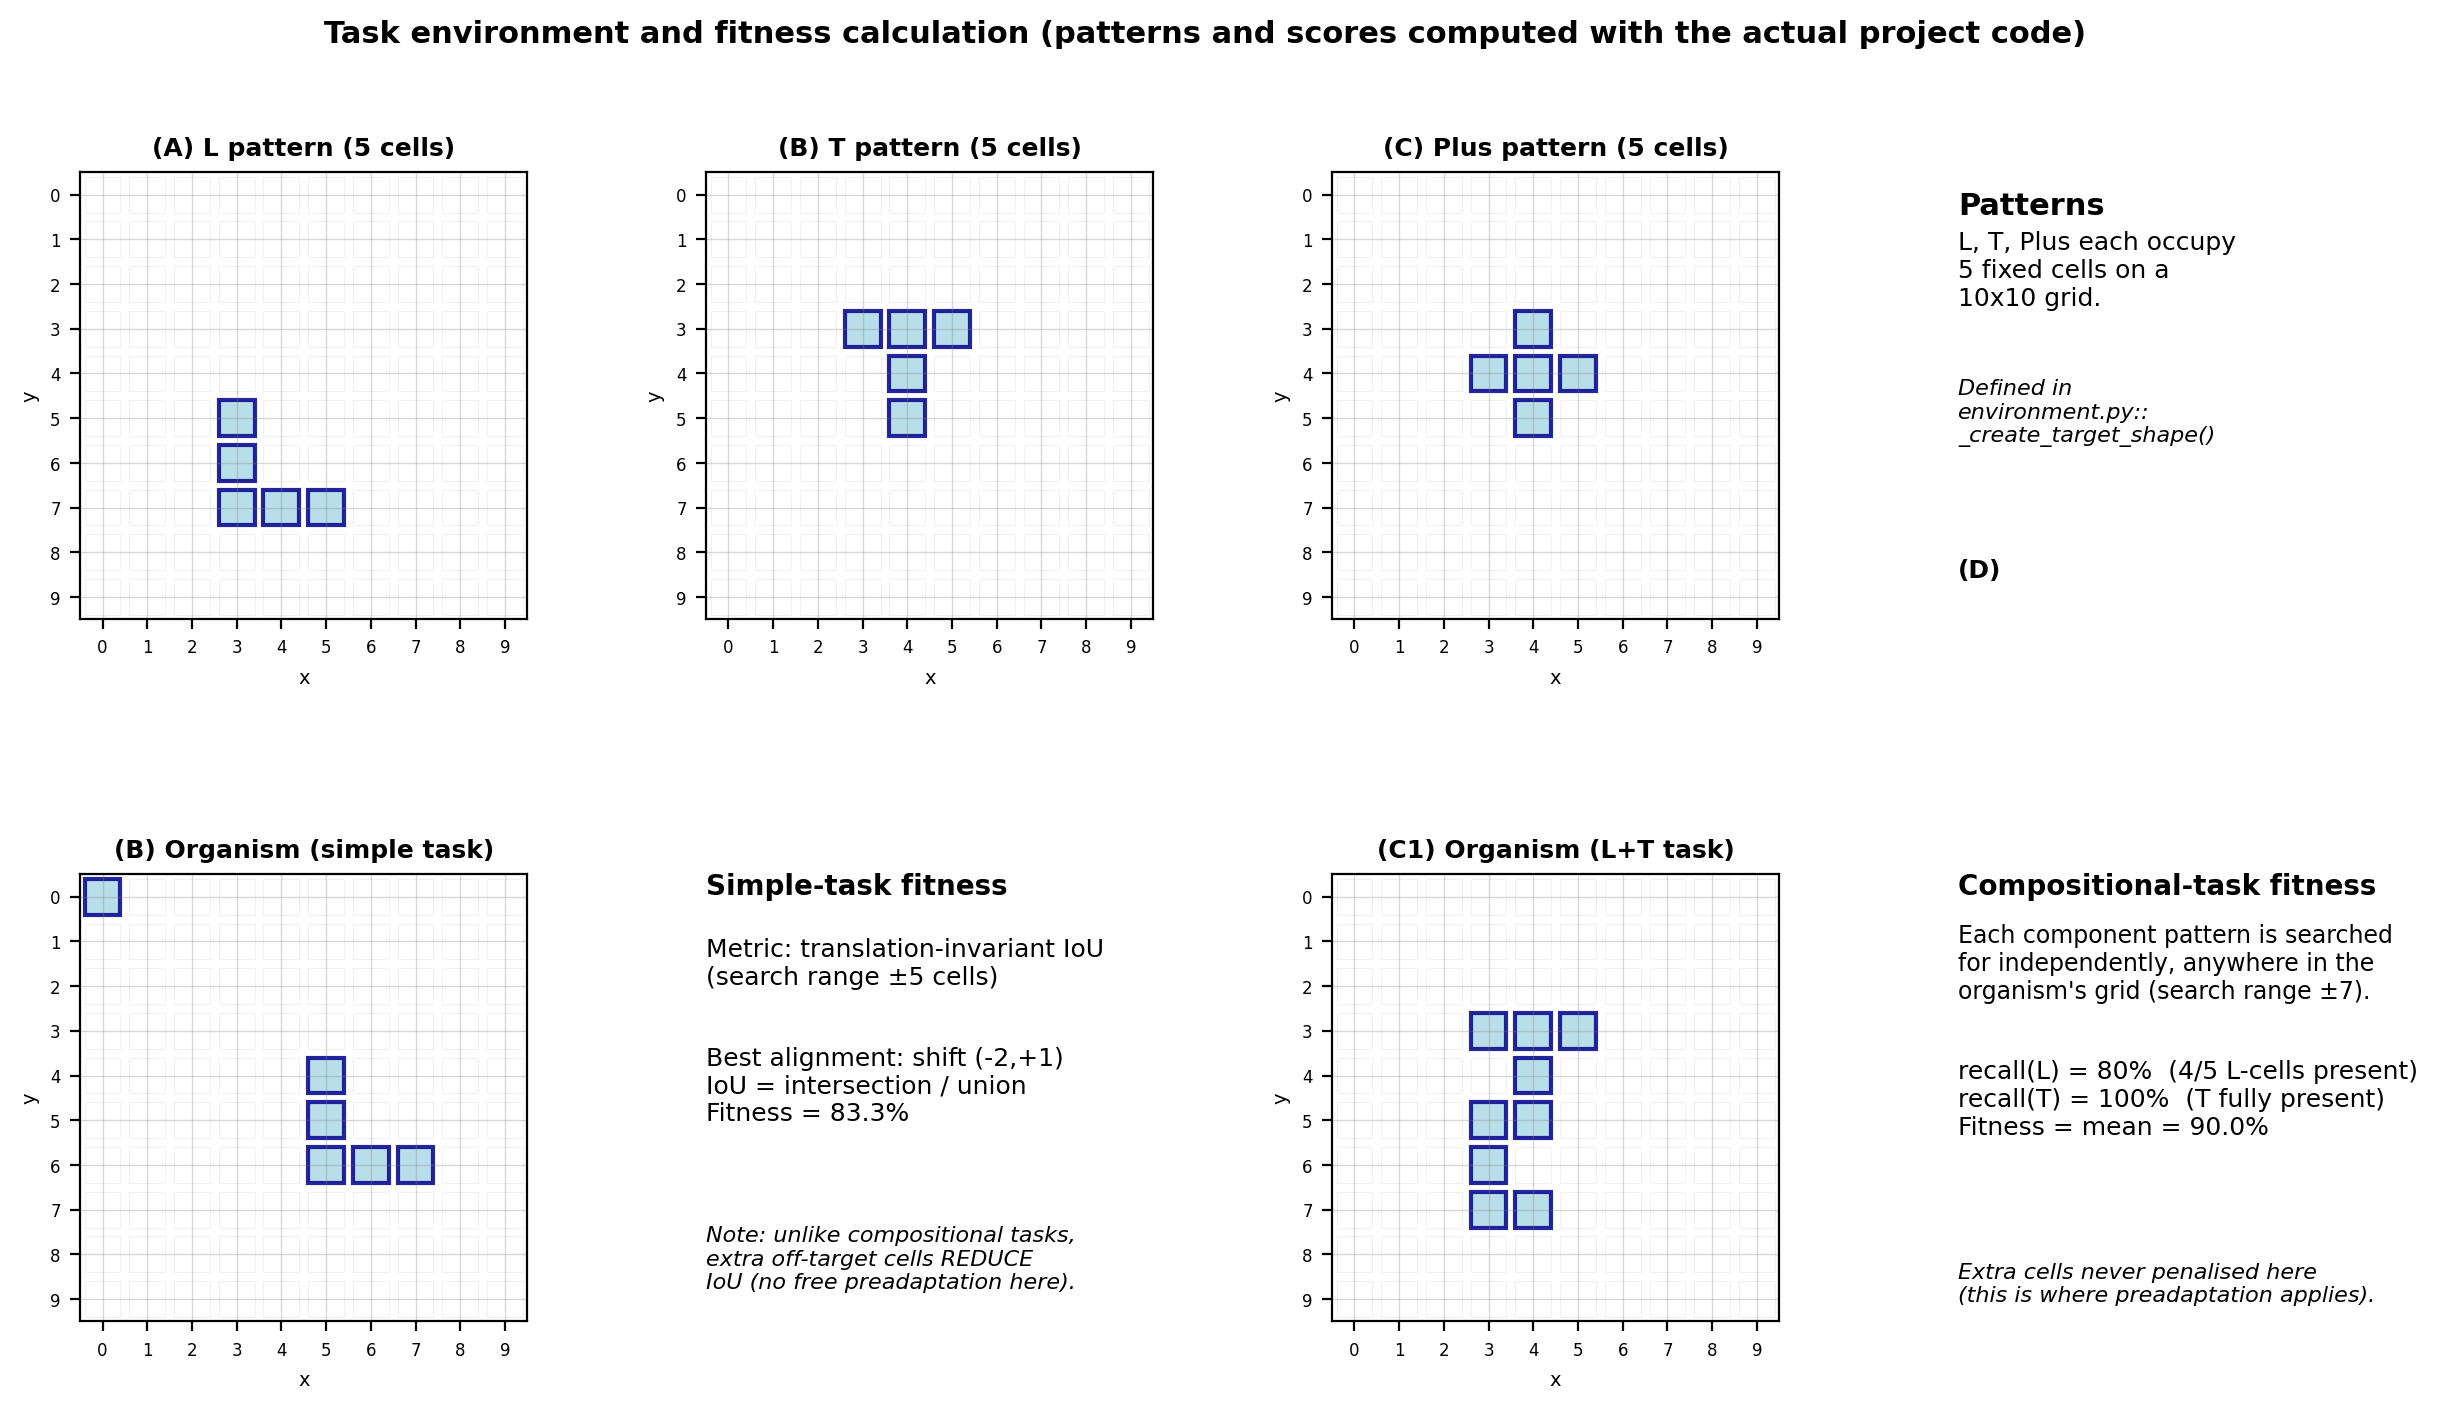
\includegraphics[width=\textwidth]{fig1_task_environment.png}
\caption{\textbf{Task environment and fitness calculation.} Top row: (A) L
pattern, (B) T pattern, (C) Plus pattern --- each occupying 5 fixed cells on
the $10\times10$ grid. Bottom row, left: a worked simple-task example. The
organism's grid (the L pattern shifted, plus one stray off-target cell) is
compared against the L pattern under translation-invariant IoU (search range
$\pm5$); the best alignment gives fitness $=83.3\%$ --- the stray cell lowers
the score, since IoU (unlike recall) penalises extra cells. Bottom row,
right: a worked compositional-task (L+T) example. The organism expresses a
complete T pattern (recall $=100\%$) and 4 of the 5 L cells (recall
$=80\%$), each found independently via translation-invariant search
($\pm7$); fitness is their mean, $90\%$. All patterns and scores in this
figure are computed directly from the project's \texttt{environment.py} and
\texttt{metrics.py}.}
\label{fig:task}
\end{figure}

\subsection{Evolutionary algorithms}

We implement three algorithms representing different inheritance mechanisms.
Each organism carries a 100-bit genome, parsed as twenty 5-bit instructions;
each instruction is read as two unsigned sub-fields that select a drawing
primitive (2 bits, taken modulo the size of a 9-primitive library -- two
lines, four corner pieces, and three junctions; since a 2-bit field cannot
exceed 3, only the first four primitives, line and corner pieces, are
reachable through the genome) and a grid position at which to stamp it
(2 bits for $x$ and 1 bit for $y$, each taken modulo the grid dimension, so
$x\in\{0,1,2,3\}$ and $y\in\{0,1\}$ in practice). An organism's
genetically-coded phenotype is the union of all 20 stamped primitives.
Genetic algorithms (GAs) simulate evolution by encoding candidate solutions as
bit-string genomes that undergo reproduction, mutation, and fitness-based
selection \citep{Holland1975,Goldberg1989}; we use this generative GA as the
computational model of the gene-centric Modern Synthesis view: only genetic
information is heritable, and evolution proceeds solely through genetic
variation and selection. We then extend this framework to test two
alternative inheritance mechanisms.

\paragraph{Gene-Centric GA (baseline).}
Pure gene-centric evolution: the phenotype above, fitness-evaluated directly,
with no lifetime modification. Reproduction is asexual (one parent per
offspring, chosen by tournament selection of size 3, with no crossover), with
the top 10\% of the population carried over unmutated each generation
(elitism) and bit-flip mutation (2\% per bit per generation) applied to the
rest. This baseline establishes that learning is necessary for these tasks,
and that the restricted reach of the genomic encoding itself (only 4 of 9
primitives, confined to the grid's top-left corner) makes a purely genomic
solution hard to find without learning or a translation search wide enough to
compensate.

\paragraph{Baldwin Effect.}
Identical genome, development, and reproduction, plus lifetime learning. Each
organism runs 20 learning trials: each trial builds a fresh candidate
phenotype from scratch by stamping 1--4 randomly chosen primitives (drawn
from the full 9-primitive library, unlike the genomic encoding) at random
grid positions, and the candidate replaces the organism's phenotype only if
its fitness exceeds the current best. Critically, whatever is discovered
during learning is \textbf{not} inherited: offspring are built from the
parent's genome plus mutation only, with no memory of what the parent
learned. Learning influences \emph{which} organisms reproduce, via its effect
on fitness and hence selection, but the learned configuration itself does not
transfer. Each generation must rediscover a good configuration independently.

\paragraph{Phenotype-First (Phenopoiesis).}
Identical genome, development, reproduction, and learning procedure to the
Baldwin Effect, plus one addition: whenever a learning trial discovers a
configuration scoring above 0.7 fitness, that configuration is appended to
the organism's \emph{epigenome} -- a growing list of learned patterns. Unlike
the genome, the epigenome is inherited by offspring in full and unmutated: a
child starts life with an exact copy of its parent's entire list of learned
patterns, in addition to whatever its own genome and lifetime learning add to
it. Before finalising its phenotype each generation, an organism also tries
every pairwise union of its inherited patterns and adopts the best-scoring
combination if it beats its current phenotype -- this is the mechanism that
lets, for example, an inherited L pattern and an inherited T pattern combine
into an L+T phenotype without relearning either component from scratch.
Figure~\ref{fig:pipeline} summarises the three mechanisms side by side.

\begin{figure}[htbp]
\centering
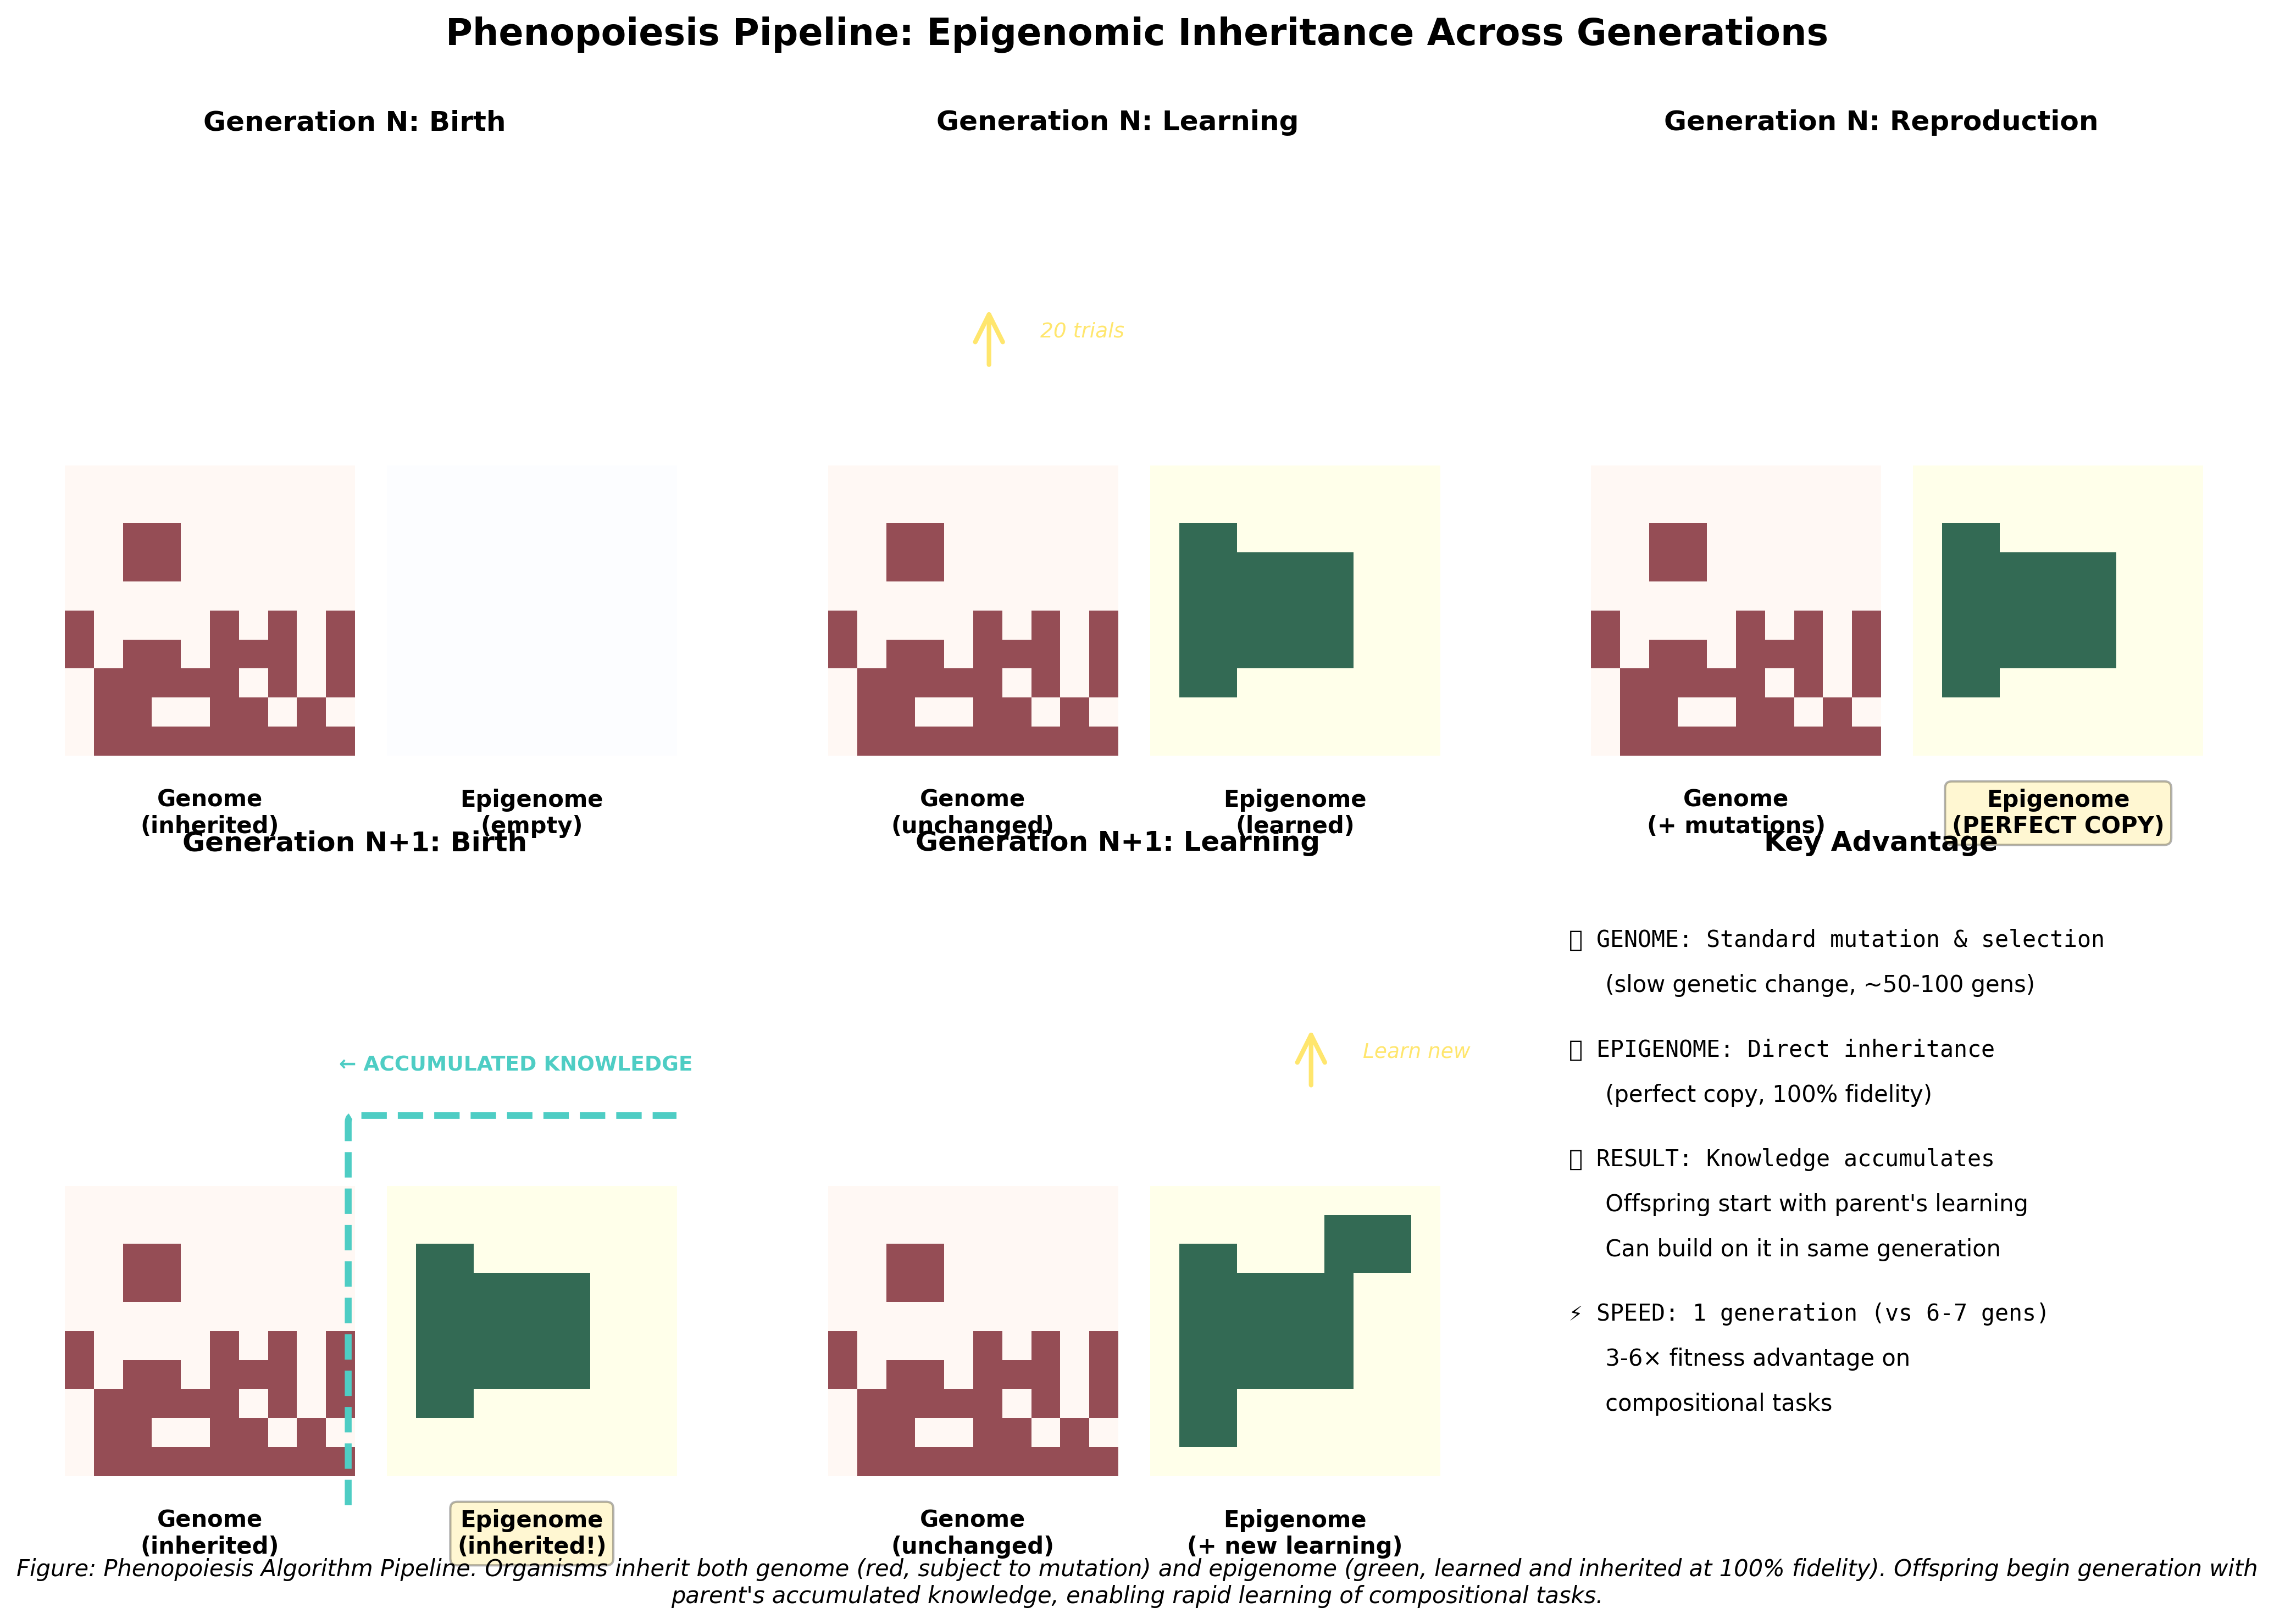
\includegraphics[width=\textwidth]{fig5_algorithm_pipeline.png}
\caption{\textbf{Algorithm pipeline.} Comparison of the inheritance and learning
loops for Gene-Centric evolution, the Baldwin Effect, and \Pheno{}. The
distinguishing step is where learned information is written and whether that
write survives reproduction.}
\label{fig:pipeline}
\end{figure}

\subsection{Experimental design}

We test three algorithms (Gene-Centric, Baldwin Effect, \Pheno{}) on six tasks
(simple: L, T, Plus; compositional: L+T, L+Plus, T+Plus). Each
task--algorithm combination is run 30 independent times with different random
seeds. Populations of 50 individuals evolve for 150 generations, allowing all
algorithms to reach a fitness plateau on simple tasks. For each run we record
final fitness at generation 150, component fitness for each pattern
(compositional tasks only), and convergence time (the generation at which
fitness first reaches 80\% of its final value). Parameters are given in
Table~\ref{tab:params}.

\begin{table}[htbp]
\centering
\small
\caption{Algorithm parameters.}
\label{tab:params}
\resizebox{\textwidth}{!}{%
\begin{tabular}{lccc}
\toprule
\textbf{Parameter} & \textbf{Gene-Centric} & \textbf{Baldwin} & \textbf{Phenopoiesis} \\
\midrule
Genome size      & 100 bits & 100 bits & 100 bits (genetic) \\
Epigenome size   & --- & --- & growing pattern list (inheritable) \\
Learning trials  & none & 20 & 20 (genetic layer fixed) \\
Learning rule    & --- & fresh random 1--4-primitive composition & fresh random 1--4-primitive composition \\
Inheritance      & genome + mutation & genome + mutation (learning reset) & genome + mutation + pattern list (100\% fidelity) \\
Selection        & tournament (size 3) & tournament (size 3) & tournament (size 3) \\
Mutation rate    & 2\% per bit & 2\% per bit & 2\% per bit (genome only) \\
Crossover        & none (asexual) & none (asexual) & none (asexual) \\
Elitism          & top 10\% & top 10\% & top 10\% \\
Population       & 50 & 50 & 50 \\
Generations      & 150 & 150 & 150 \\
Replicates       & 30 & 30 & 30 \\
\bottomrule
\end{tabular}%
}
\end{table}

\subsection{Statistical analysis}

We apply one-way ANOVA for each task comparing the three algorithms, with
Bonferroni correction ($\alpha = 0.05$). ANOVA assumptions are checked with
Shapiro--Wilk (normality) and Levene's test (homogeneity of variance); where
violated, Welch's $F$-test is used. For pairwise Baldwin vs.\ \Pheno{}
comparisons we use Welch's $t$-test with Cohen's $d$ effect size. The standard
deviation of fitness characterises consistency: low s.d.\ indicates
deterministic learning, high s.d.\ stochastic exploration.

\subsection{Computational details}

All algorithms are implemented in Python 3.9 using standard libraries only.
Reproducibility was verified by re-running three representative conditions and
confirming identical results under identical seeds. Total computation was
approximately 48 hours on a standard laptop processor for all 540 runs
(30 replicates $\times$ 6 tasks $\times$ 3 algorithms).

% ============================================================================
\section{Results}

\subsection{Simple tasks: inheritance is irrelevant}

On simple learning tasks (L, T, or Plus alone), both the Baldwin Effect and
\Pheno{} reach 100\% fitness while the Gene-Centric GA achieves only 56--59\%
(Table~\ref{tab:simple}, Figure~\ref{fig:simple}), confirming that learning is
essential. Baldwin and \Pheno{} show no significant difference
($p = 0.559$, $d = 0$), indicating that epigenomic write-back provides no
additional advantage when phenotypic plasticity alone suffices.

\begin{table}[htbp]
\centering
\caption{\textbf{Simple learning task results} (mean fitness $\pm$ s.d., $n = 30$).
Gene-Centric establishes that learning is essential. Baldwin and \Pheno{} both
reach 100\% fitness with no difference between them, showing the inheritance
mechanism is irrelevant on simple tasks.}
\label{tab:simple}
\begin{tabular}{lccc}
\toprule
\textbf{Task} & \textbf{Gene-Centric} & \textbf{Baldwin} & \textbf{Phenopoiesis} \\
\midrule
L alone    & $0.57 \pm 0.28$ & $1.00 \pm 0.00$ & $1.00 \pm 0.00$ \\
T alone    & $0.59 \pm 0.31$ & $1.00 \pm 0.00$ & $1.00 \pm 0.00$ \\
Plus alone & $0.56 \pm 0.25$ & $1.00 \pm 0.00$ & $1.00 \pm 0.00$ \\
\bottomrule
\end{tabular}
\end{table}

\begin{figure}[htbp]
\centering
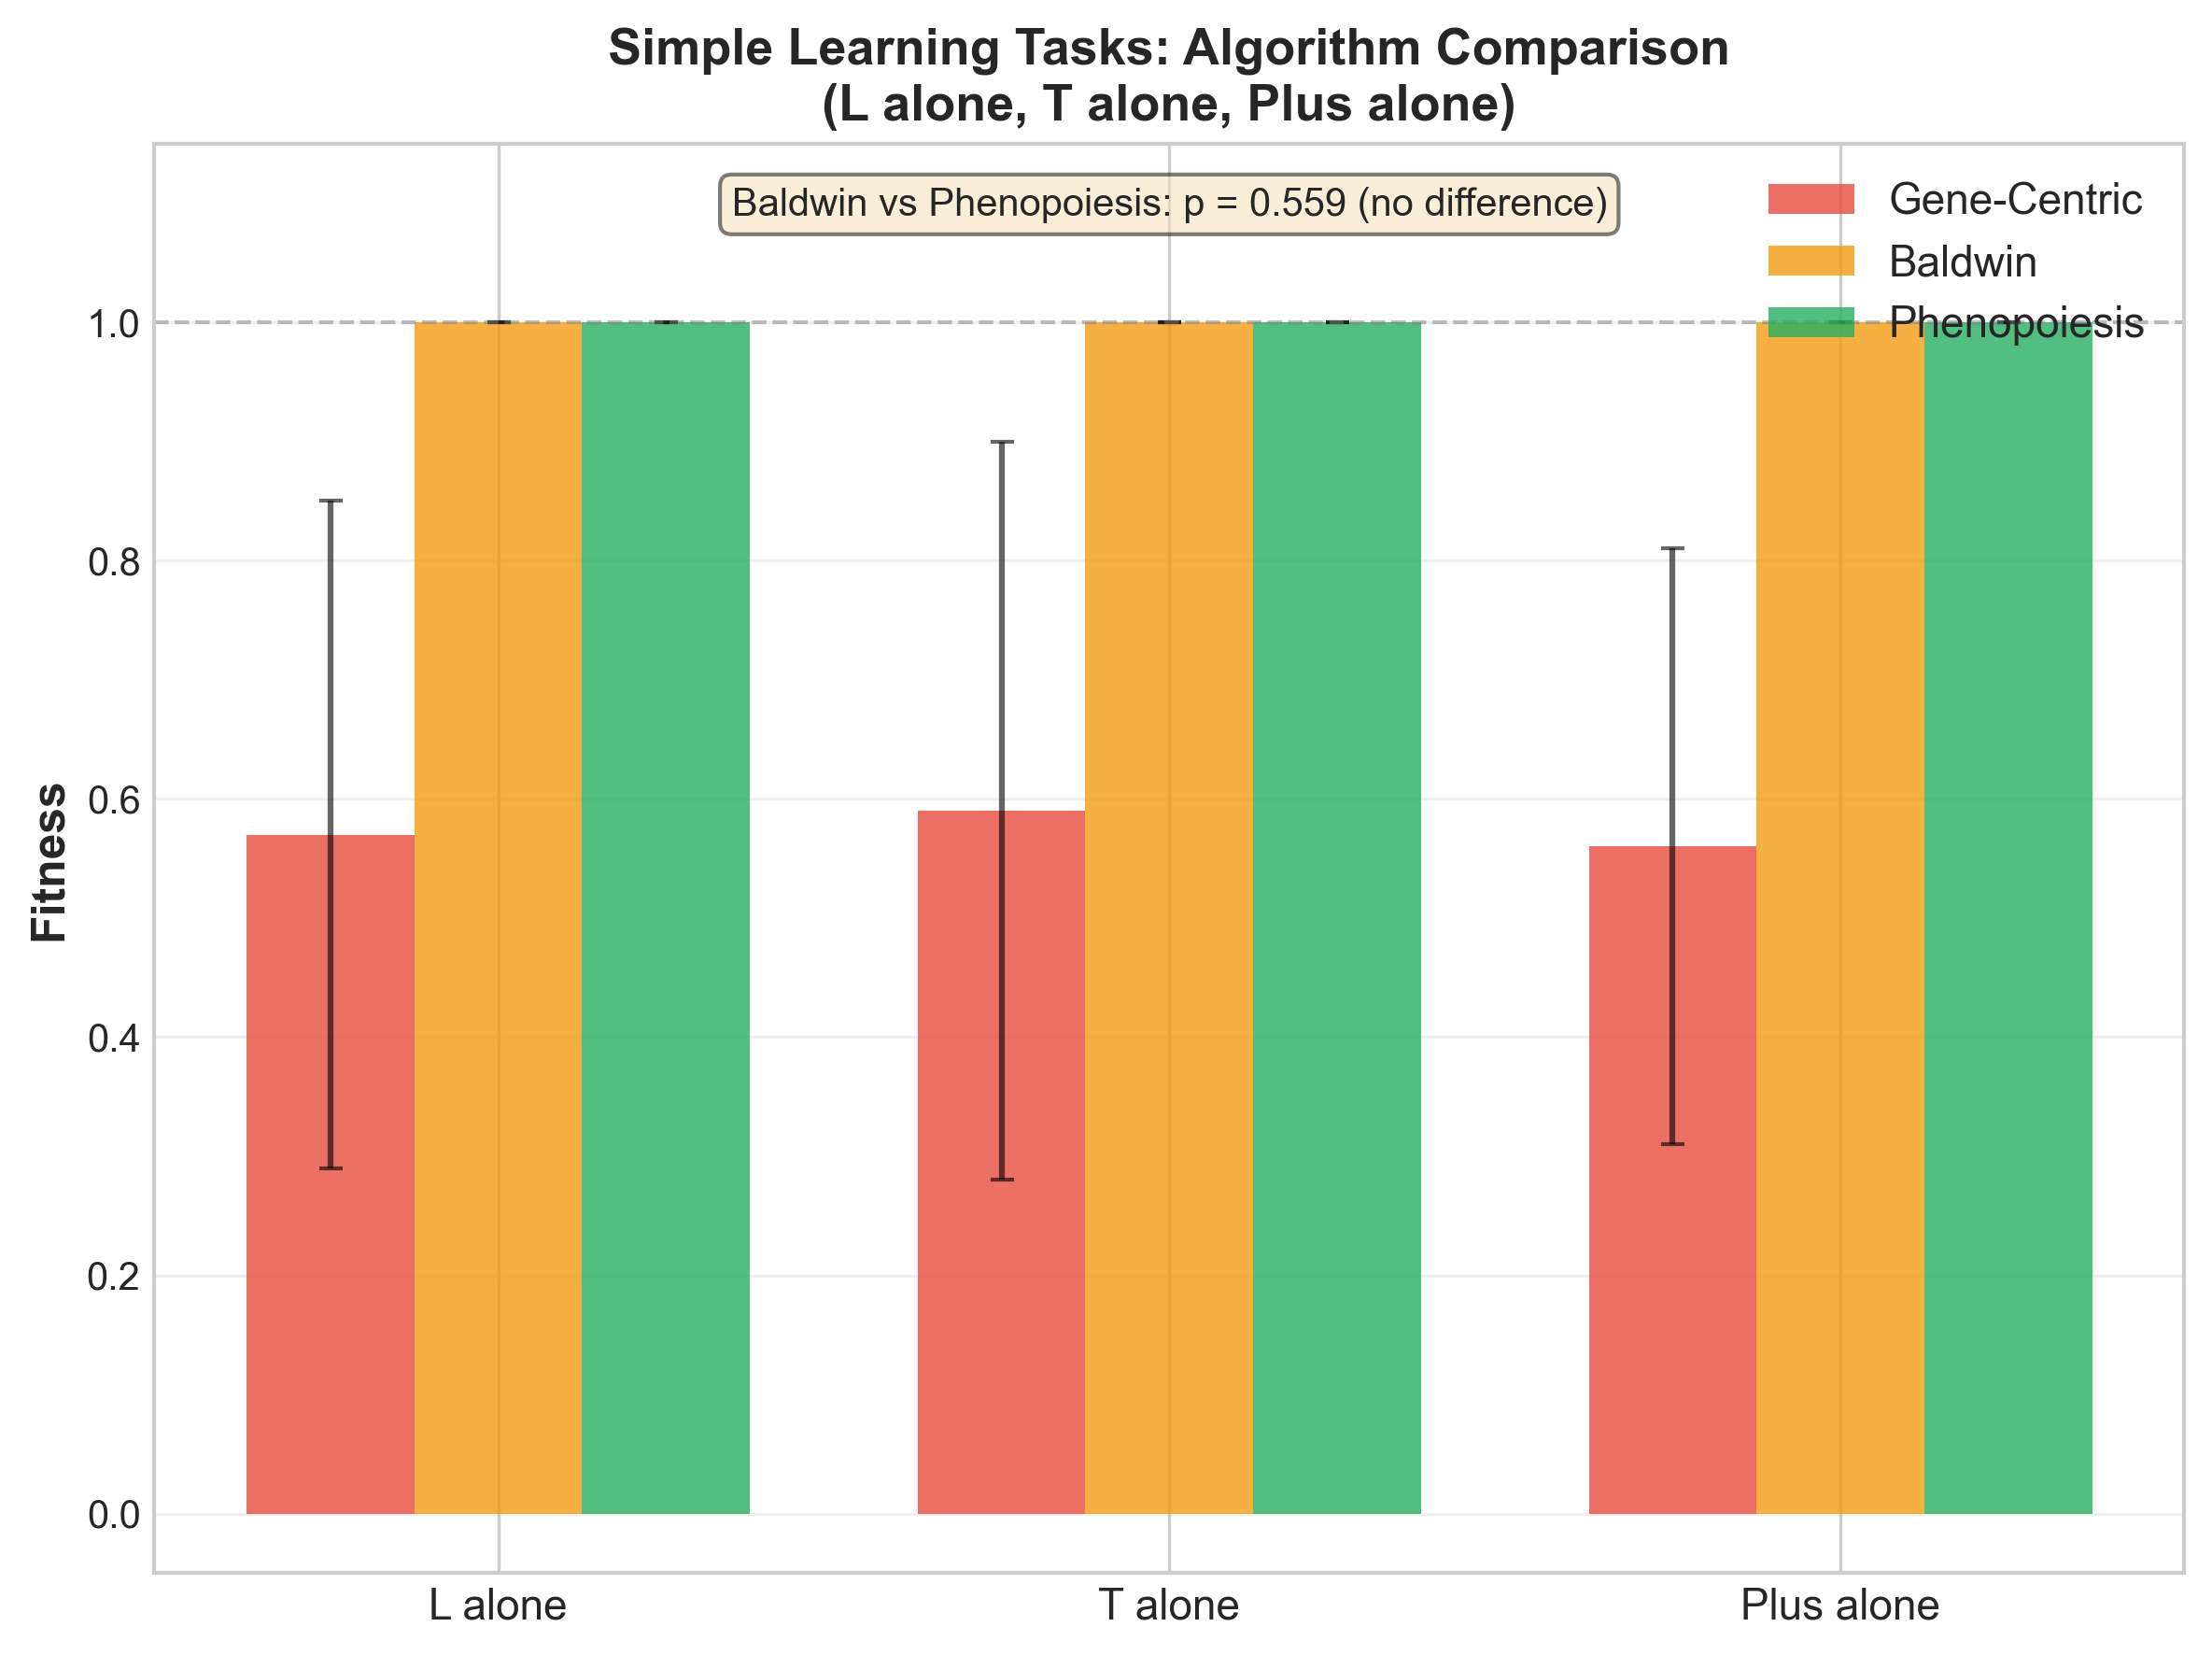
\includegraphics[width=\textwidth]{fig2_simple_tasks.png}
\caption{\textbf{Simple learning tasks: algorithm comparison.} Mean fitness
$\pm$ s.d.\ for Gene-Centric (red), Baldwin Effect (orange), and \Pheno{}
(green) on single-pattern tasks. Gene-Centric achieves only 56--59\% fitness (no
learning), while Baldwin and \Pheno{} both reach 100\% with no significant
difference ($p = 0.559$, $d = 0$), showing that the inheritance mechanism is
irrelevant when learning alone suffices. Error bars: s.d.\ over 30 runs.}
\label{fig:simple}
\end{figure}

\subsection{Compositional tasks: a 3--6$\times$ advantage}

On learnable compositional tasks (L+T and T+Plus) the results diverge sharply
(Table~\ref{tab:comp}, Figure~\ref{fig:comp}). \Pheno{} achieves 3.0--6.0$\times$
higher fitness than the Baldwin Effect ($p < 0.001$, $d > 3.4$), with perfect
reproducibility on T+Plus (all 30 runs identical). Learning trajectories show
this advantage emerging as organisms evolve: \Pheno{} accelerates rapidly with
low variance, while the Baldwin Effect improves gradually and stochastically
(Figure~\ref{fig:traj}, left and centre panels). The Baldwin Effect shows high
variance and near-total failure---it cannot accumulate knowledge across
generations. \Pheno{} succeeds consistently, demonstrating that direct
epigenomic inheritance lets organisms inherit learned patterns and build on them
in subsequent generations.

\begin{table}[htbp]
\centering
\caption{\textbf{Compositional learning task results} (mean fitness $\pm$ s.d.,
$n = 30$). Baldwin Effect (selection-based) vs.\ \Pheno{} (epigenomic
write-back). Learnable compositional tasks (L+T, T+Plus) show a large \Pheno{}
advantage; the hard task (L+Plus) shows none, revealing the limits of extended
agency.}
\label{tab:comp}
\resizebox{\textwidth}{!}{%
\begin{tabular}{lcccccc}
\toprule
\textbf{Task} & \textbf{Baldwin} & \textbf{Phenopoiesis} & \textbf{Advantage} & \textbf{F} & \textbf{p} & \textbf{Cohen's d} \\
\midrule
L+T     & $0.254 \pm 0.196$ & $0.772 \pm 0.075$ & 3.0$\times$ & 177.08 & $<0.001$ & 3.44 \\
T+Plus  & $0.086 \pm 0.123$ & $0.517 \pm 0.000$ & 6.0$\times$ & 358.56 & $<0.001$ & 4.89 \\
L+Plus  & $0.177 \pm 0.149$ & $0.189 \pm 0.156$ & 1.1$\times$ & 0.07   & 0.789    & 0.08 \\
\bottomrule
\end{tabular}%
}
\end{table}

\begin{figure}[htbp]
\centering
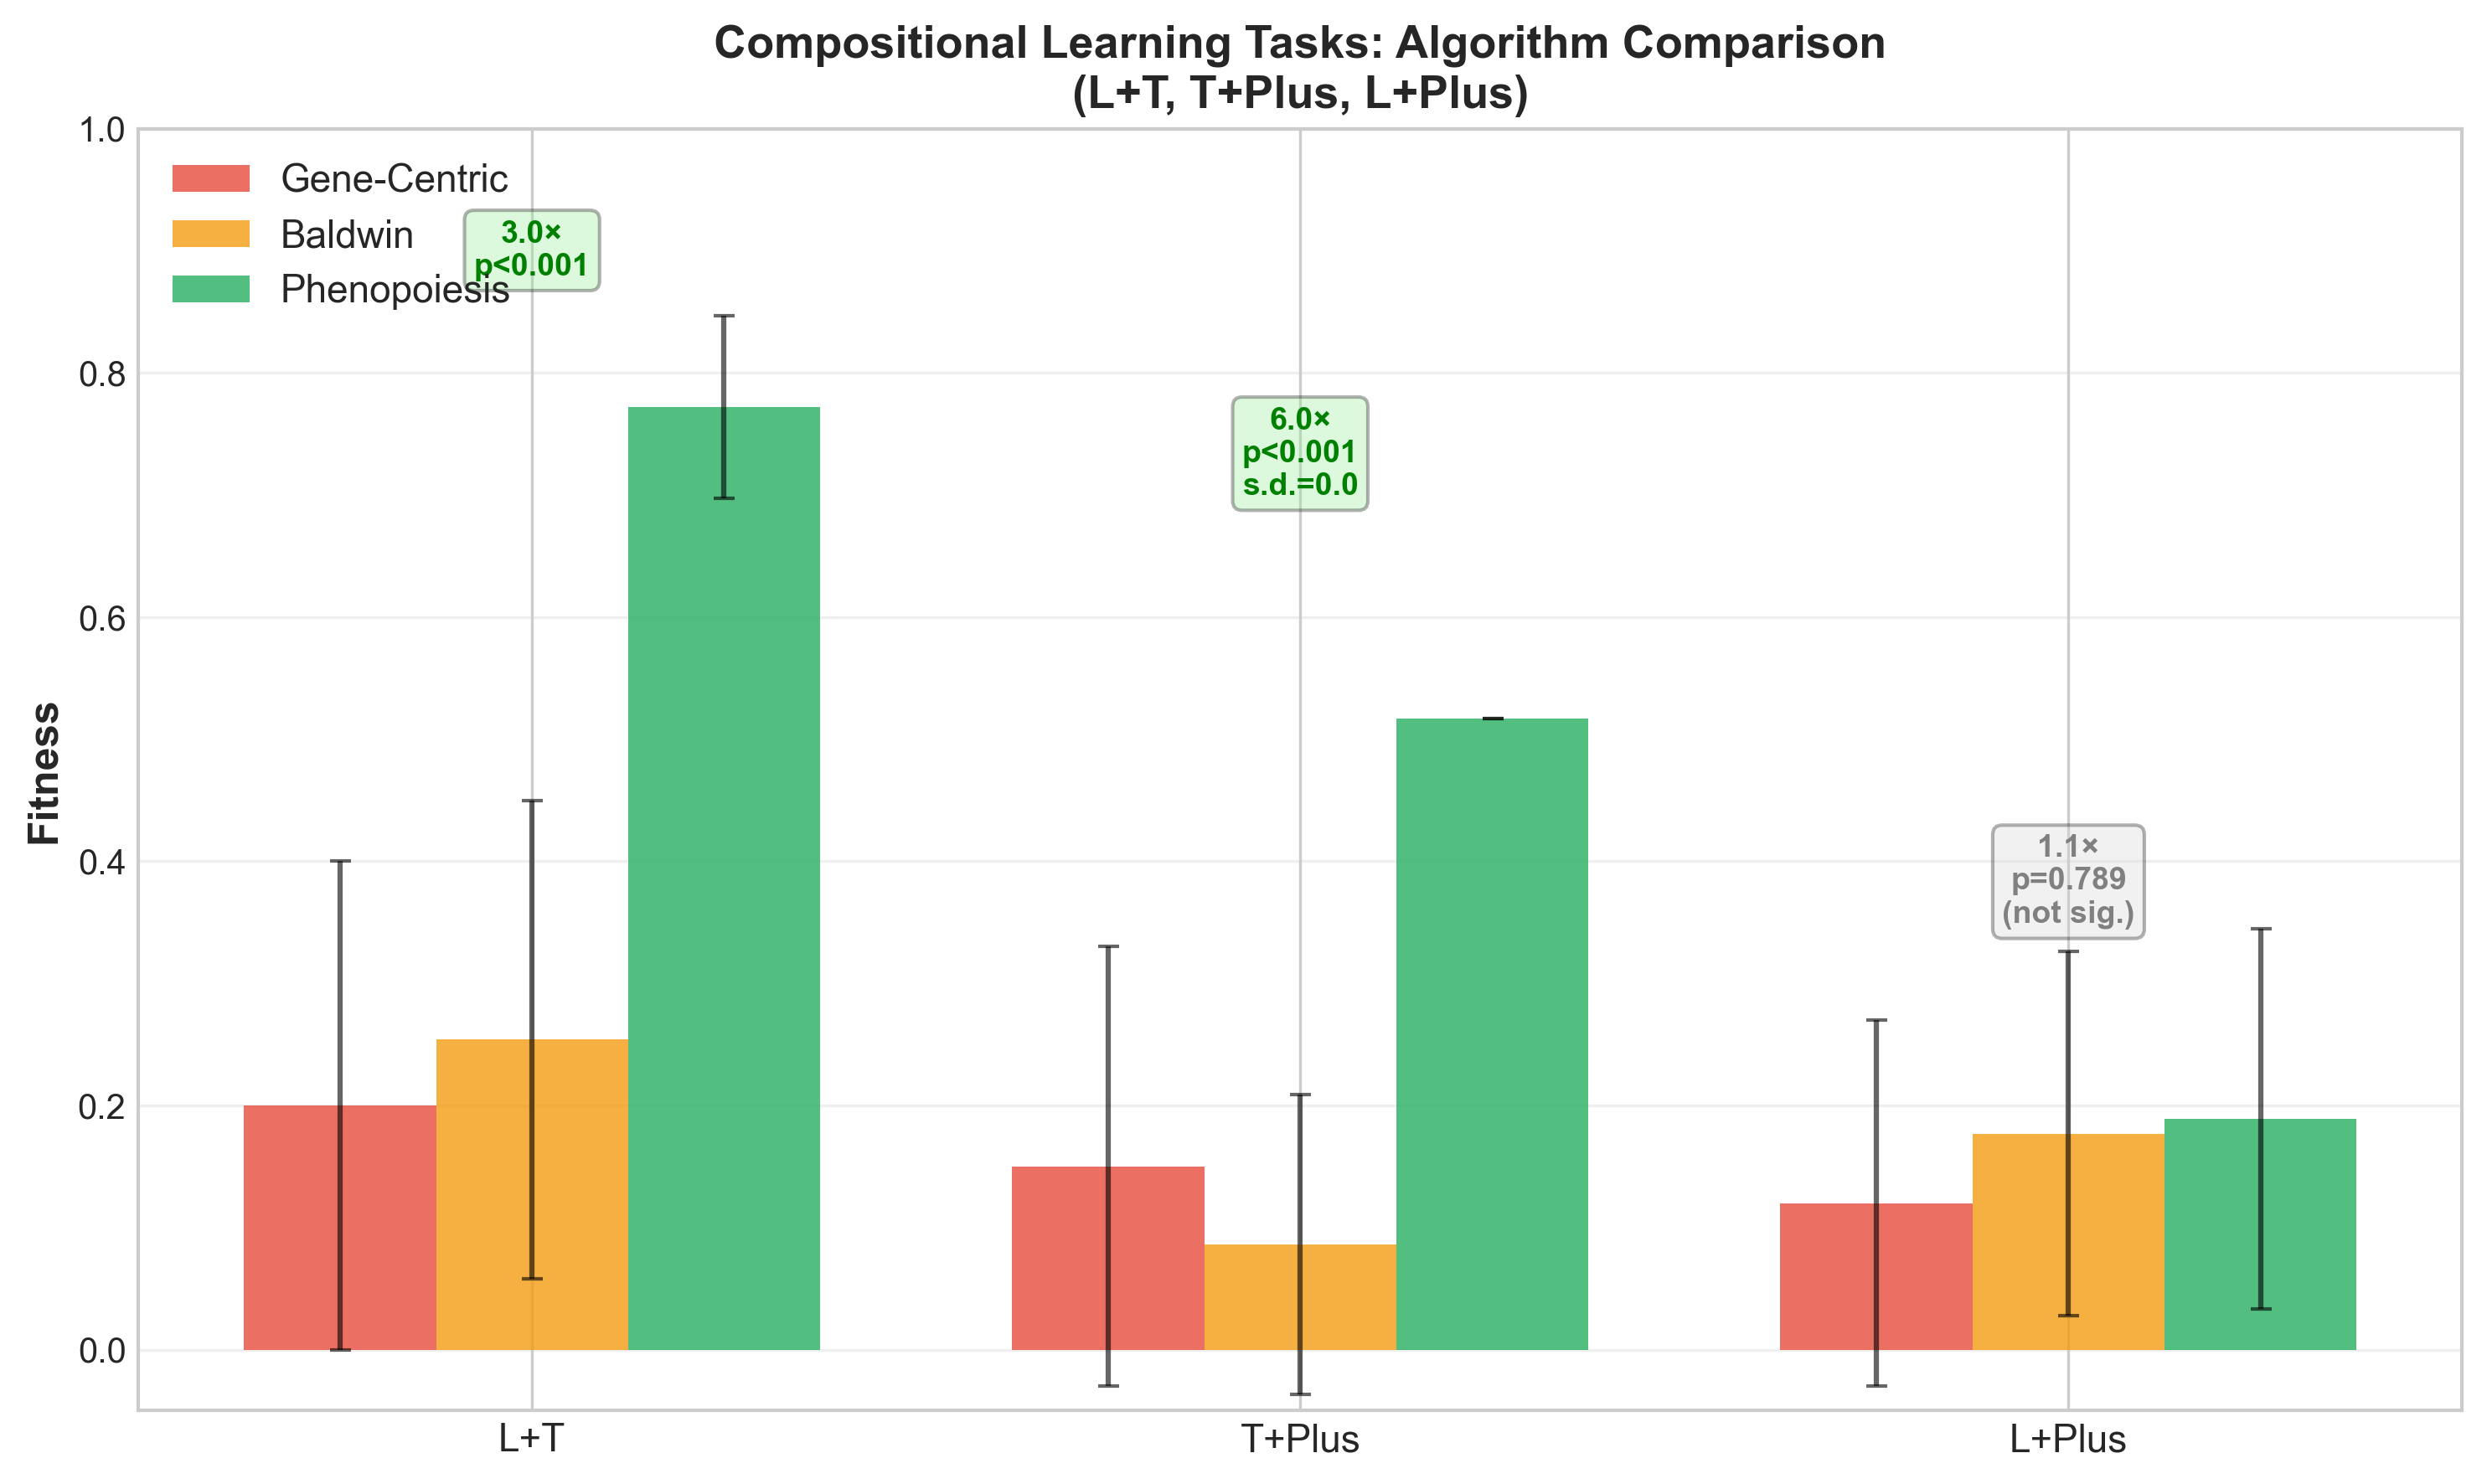
\includegraphics[width=\textwidth]{fig3_compositional_tasks.png}
\caption{\textbf{Compositional learning tasks: all three algorithms.} Mean
fitness $\pm$ s.d.\ for Gene-Centric (red), Baldwin Effect (orange), and
\Pheno{} (green) across three tasks requiring the simultaneous learning of two
patterns. (Left) L+T: \Pheno{} achieves 3.0$\times$ higher fitness than Baldwin
($p < 0.001$). (Centre) T+Plus: \Pheno{} achieves 6.0$\times$ higher fitness with
perfect reproducibility (s.d.\ $= 0.0$, all 30 runs identical, $p < 0.001$).
(Right) L+Plus: no advantage for either mechanism ($p = 0.789$) due to geometric
pattern incompatibility. Error bars: $\pm 1$ s.d.}
\label{fig:comp}
\end{figure}

\subsection{Limits: geometric incompatibility defeats every mechanism}

The hard compositional task (L+Plus) shows no advantage for either mechanism
($p = 0.789$), with both algorithms failing to reach high fitness
(Figure~\ref{fig:comp}, right panel; Figure~\ref{fig:traj}, right panel, showing
convergence at $\approx 18\%$). Extended agency has limits: both methods fail
equally when pattern components geometrically interfere. Extended agency
provides an evolutionary advantage precisely when organisms must accumulate
learned knowledge across generations---but only when the problem decomposes into
independently learnable components.

\begin{figure}[htbp]
\centering
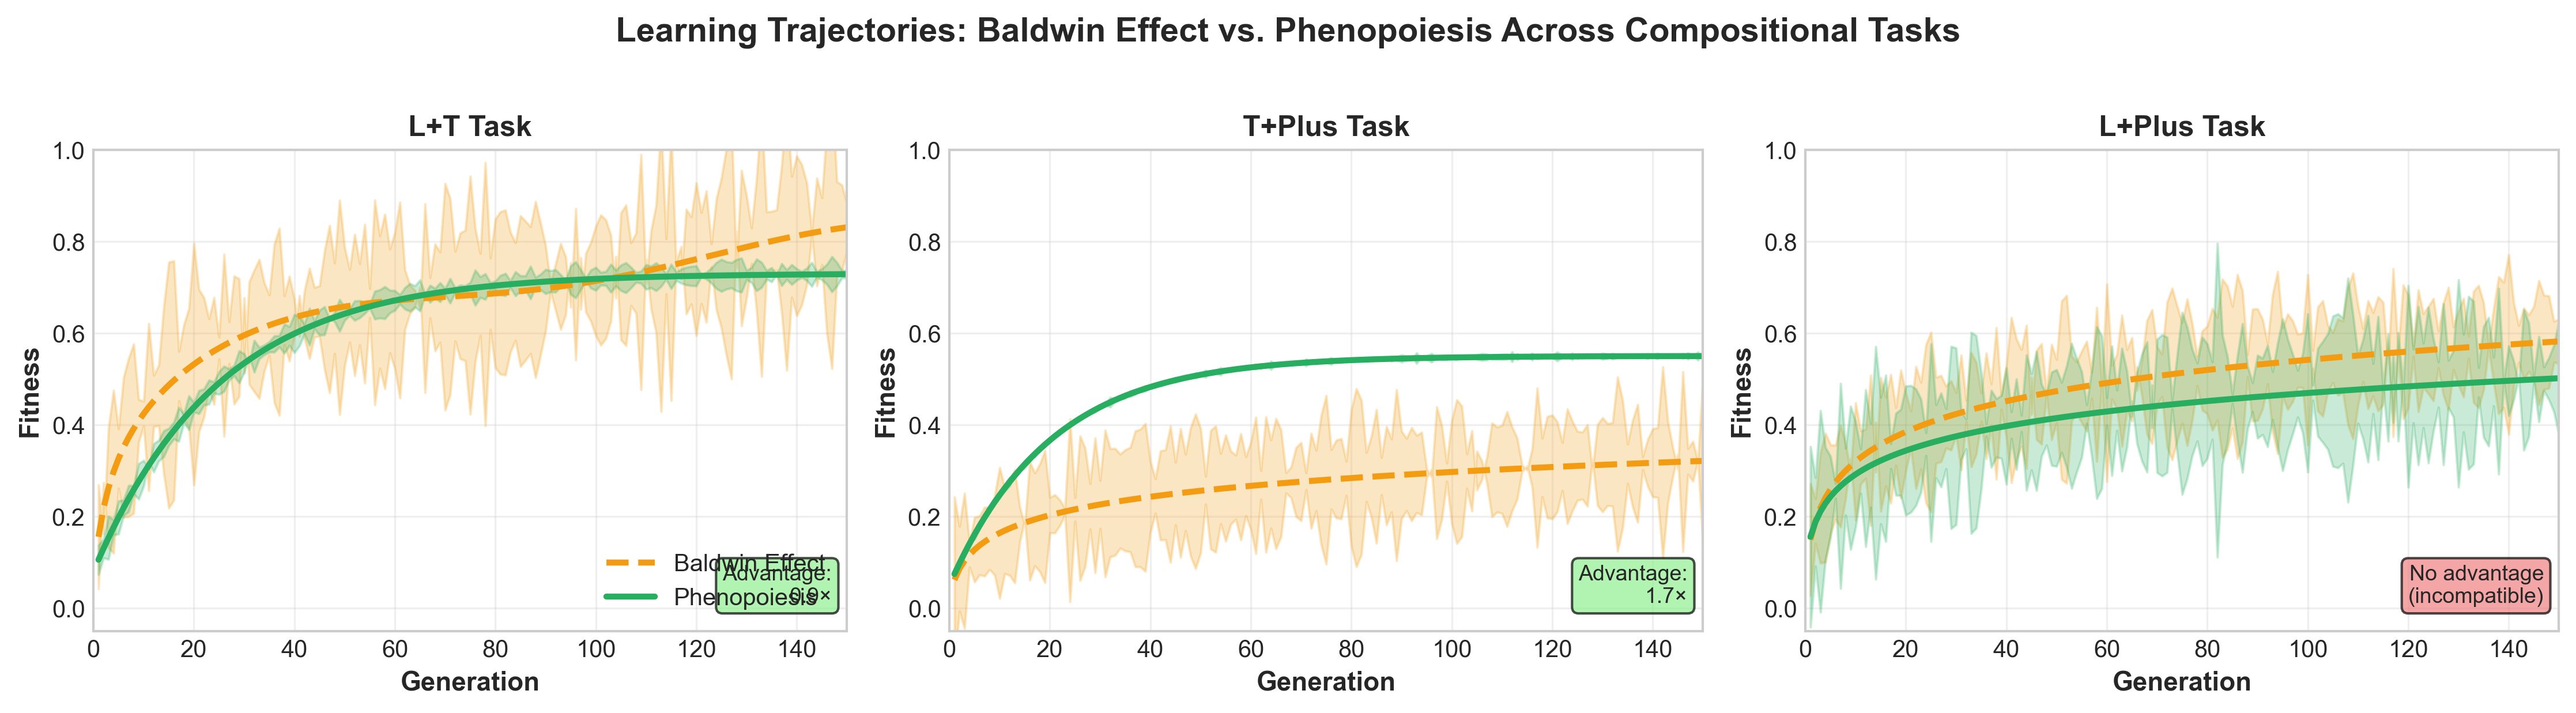
\includegraphics[width=\textwidth]{fig4_learning_trajectories.png}
\caption{\textbf{Learning trajectories across all compositional tasks.} Mean
fitness over 150 generations for the Baldwin Effect (orange, dashed) and
\Pheno{} (green, solid), with shaded $\pm 1$ s.d.\ regions. (Left) L+T: \Pheno{}
shows early acceleration and low variance; Baldwin improves gradually and
stochastically. (Centre) T+Plus: \Pheno{} is perfectly deterministic
(s.d.\ $= 0.0$); Baldwin shows high variance and minimal learning. (Right)
L+Plus: both mechanisms plateau at similar low fitness ($\approx 18\%$),
revealing geometric incompatibility between the patterns.}
\label{fig:traj}
\end{figure}

% ============================================================================
\section{Discussion}

Our results provide the first quantitative test of Denis Noble's hypothesis that
organisms possess direct read--write access to their heredity. We find strong,
statistically robust evidence that epigenomic write-back dramatically
accelerates evolutionary learning on compositional tasks. On learnable
compositional problems (L+T and T+Plus), \Pheno{} achieved 3.0--6.0$\times$
higher fitness than the Baldwin Effect ($p < 0.001$, Cohen's
$d = 3.44$--$4.89$). Perfect reproducibility on T+Plus (all 30 runs identical,
s.d.\ $= 0.0$) reveals that inherited learning enables deterministic, repeatable
evolution---a qualitative shift away from the random search of selection-only
mechanisms. The results also set clear boundaries: on simple tasks, write-back
provides no acceleration; on hard compositional tasks, both mechanisms fail
equally.

\subsection{Direct write-back versus selection-based agency}

The Extended Evolutionary Synthesis recognises that organisms actively shape
evolution through niche construction, developmental plasticity, and learning.
Yet EES remains fundamentally selection-based: learning influences the
phenotype, which alters selection pressure, which eventually reshapes genes over
many generations---an indirect, slow process. Noble's proposal is different in
kind: organisms do not merely influence evolution through selection, they
actively compose their evolution by writing learned patterns directly into
heritable epigenomic form.

Our data quantify that distinction. The gap appears only when knowledge must
accumulate across generations---precisely where Noble's mechanism should matter.
The Baldwin Effect, while more powerful than gene-only evolution, cannot match
the speed of direct write-back because each generation must rediscover prior
solutions before learning new ones. Three regimes emerge:

\begin{itemize}
  \item \textbf{Simple tasks} ($1.0\times$): inheritance is irrelevant when a
        single pattern can be learned within one generation.
  \item \textbf{Learnable compositional tasks} ($3$--$6\times$): inherited
        knowledge dramatically accelerates evolution; offspring inherit parents'
        learned solutions and focus effort on new patterns.
  \item \textbf{Hard compositional tasks} ($1.0\times$): when components
        geometrically interfere, neither mechanism helps---decomposability, not
        the inheritance mechanism, determines solvability.
\end{itemize}

\subsection{Compositionality as the central constraint}

Real epigenetic inheritance (DNA methylation, histone modifications) persists
through meiosis and transmits acquired information across generations
\citep{Pembrey2006,WaterlandJirtle2007}. Our model assumes 100\% fidelity
copying (real systems degrade) and artificial binary patterns (real learning is
continuous), but the core principle---learned regulatory changes inherited with
near-complete fidelity---is biologically grounded.

Compositionality emerges as the central constraint on evolutionary innovation,
because major transitions require solving multiple distinct problems whose
solutions must coexist \citep{MaynardSmith1995}. The prokaryote-to-eukaryote
transition requires compartmentalisation, a nuclear envelope, chromatin
organisation, nuclear transport, and gene regulation---each layer building on
and compatible with the previous ones. Unicellular-to-multicellular transitions
involve cell adhesion, signalling, differentiation, and morphogenesis, where
each layer enables rather than prevents subsequent layers. Inherited knowledge
accumulation lets organisms discover one layer, inherit that solution, then
discover the next, avoiding exponential search.

Not all paired problems have this structure, and our L+Plus failure is
informative. The L and Plus patterns geometrically overlap on the
$10\times10$ grid, competing for the same cells; achieving perfect fitness for
both simultaneously is impossible. The patterns are incompatible constraints,
not sequential layers. This incompatibility cannot be overcome by inheritance or
any learning mechanism---it is a property of the problem structure, not a
limitation of extended agency. The distinction between compatible sequential
layers and incompatible simultaneous constraints explains both evolutionary
successes and failures.

\subsection{Limitations and future work}

We tested artificial visual tasks, not ecological complexity; modelled binary
learning, not continuous acquisition; assumed perfect epigenomic fidelity, not
real degradation; and examined asexual lineages, not sexual recombination.
Despite these simplifications, the 3--6$\times$ advantage on learnable
compositional tasks demonstrates that epigenomic inheritance accelerates
solutions when the problem structure permits incremental construction. Future
work should introduce realistic epigenomic decay rates, examine interactions
with sexual reproduction, scale to continuous-valued learning, and characterise
which biological innovations have compositionally compatible versus incompatible
structure.

% ============================================================================
\section{Conclusion}

We demonstrated that heritable epigenomic inheritance of learned patterns
accelerates evolutionary problem-solving 3--6 fold on compositional tasks. This
acceleration arises because offspring inherit their parents' learned solutions
and build upon them rather than rediscovering them each generation. It applies
specifically when problems decompose into sequentially compatible layers---each
layer enabling rather than preventing the next. On simple tasks, inheritance
provides no acceleration; on incompatible problems, no mechanism helps. This
specificity is what makes the result mechanistic rather than merely
philosophical: organisms that transmit learned epigenomic states to offspring
can solve compositional problems orders of magnitude faster than organisms
relying solely on genetic evolution and selection.

% ============================================================================
\section*{Data and code availability}

All data, code, and figures are available at
\begin{center}
\url{https://github.com/drnamlabs-gif/phenotype-first-evolution}
\end{center}
\noindent
The repository contains the complete Python implementation of all three
algorithms (Gene-Centric GA, Baldwin Effect, \Pheno{}), the experimental
pipeline, raw results from all 540 runs as CSV, the figure-generation scripts,
and the LaTeX source of this preprint.

\section*{Author contributions}

N.H.L.\ conceived the study, implemented the algorithms, ran the experiments,
analysed the data, and wrote the manuscript.

% ============================================================================
\bibliography{references}

\end{document}
